\documentclass[11pt]{article}

\usepackage[english]{babel}
\usepackage[utf8]{inputenc}
\usepackage{amsmath}
\usepackage{amssymb}
\usepackage{graphicx}
\usepackage[colorinlistoftodos]{todonotes}
\usepackage{listings,multicol}
\usepackage{textcomp}
\usepackage{hyperref}

\setlength{\oddsidemargin}{0.5cm} \setlength{\evensidemargin}{0cm}
\setlength{\textwidth}{16cm} \setlength{\textheight}{23cm}
\setlength{\topmargin}{-0.5cm}
\textheight 21.5cm


\begin{document}

\title{Test1 F NUMERICO 220028 UBB}

{\begin{minipage}{2cm}
\hspace*{1cm}
\includegraphics[width=0.6\textwidth]{escubo-ubb.eps}
\end{minipage}
\begin{minipage}{12cm}
\small
{\bf \rm 
{
\begin{center}
{\footnotesize UNIVERSIDAD DEL B\'IO-B\'IO} \\
{\scriptsize FACULTAD DE CIENCIAS}  \\
{\scriptsize DEPARTAMENTO DE MATEM\'ATICA}  \\
{\scriptsize Profesor:  Franco Milanese}\\
{\scriptsize Segundo Semestre de 2015}
\end{center}
}}
\end{minipage}}
{\begin{minipage}{2cm}
\hspace*{-0.5cm}\vspace*{-0.05cm}
\includegraphics[width=0.7\textwidth]{escudo-dmat.eps}
\end{minipage}}

\hspace*{-1,5cm}\rotatebox[origin=c]{90}{\begin{picture}(0,0)
\put(0,7){\makebox(9,-13)[l]{\hspace*{-6.5in} \bf \it Departamento de Matem\'atica - Universidad del B\'io-B\'io - 2015}}
\end{picture}}

\vspace*{0.5cm} \centerline {\bf\underline{Test 1 Formativo, M\'etodos Num\'ericos I 220028 }}
%\centerline{\textrm{Martes 1 de noviembre 2015.}}  \vspace{0.2cm}


\begin{center}
 \begin{tabular}{p{0.7\textwidth}p{0.3\textwidth}}
	\textbf{Nombre:}   &\textbf{Carrera:}\\
	\textbf{Profesor:} & \textbf{ RUT:}
 \end{tabular}
 \\
 \vspace{0.2cm}
 \begin{tabular}{||p{2cm}|p{2cm}||p{2cm}||}
 \hline
 Pregunta 1 &  Pregunta 2  &     Total\\
 \hline

  \vspace{1.5cm} & &     \\
 \hline
 \end{tabular}
 \end{center}
 Enviar documentos solicitados en el formato solicitado a \textbf{veranonumerico@gmail.com}.

\begin{enumerate}
\item (20 pt) Descargue el archivo ubicado en 
\begin{center}
\url{http://www.udec.cl/~fmilanese/Indultos2006-2012.csv}
\end{center}
este contiene el detalle de los indultos concedidos a criminales entre los a\~nos 2006 y 2012 en Chile. 
\begin{enumerate}
	\item En un rutero llamado \texttt{indultos.m} lleve a Matlab el archivo descargado usando el comando \texttt{dlmread()}. 
    \item En el mismo rutero grafique la cantidad de indultos otorgados por a\~no.
    \item Grabe la gr\'afica generada como \texttt{indultosporanho.jpg}
\end{enumerate}
Adjunte el programa \texttt{indultos.m} y la gr\'afica \texttt{indultosporanho.jpg} al correo.

\textquestiondown C\'ual es el crimen con mayor cantidad de indultos?.

\fbox{ \begin{minipage}{\textwidth}  

%TR\'AFICO IL\'ICITO DE ESTUPEFACIENTES 
\hfill\vspace{1cm} 
\end{minipage} } 

\textbf{Desarrollo: } 
% \begin{enumerate}
% \item El fichero descargado es  
% \begin{verbatim}
% ANHO,SEXO,EDAD,DELITO,MOTIVO
% 2006,M,26,HOMICIDIO SIMPLE + ROBO CON INTIMIDACION + MALTRATO DE OBRA A CARABINEROS,RAZONES HUMANITARIAS 
% 2006,F,35,TRAFICO ILICITO DE ESTUPEFACIENTES,RAZONES HUMANITARIAS 
% 2006,M,47,ROBO CON FUERZA EN LUGAR NO HABITADO (FRUSTRADO),
% 2006,M,42,BIGAMIA,SITUACION FAMILIAR
% 2006,M,31,ROBO CON INTIMIDACION,POSIBILIDAD DE POSTULACION A BENEFICIOS
% 2006,M,32,ROBO CON INTIMIDACION,REINSERCION SOCIAL
% 2006,F,39,TRAFICO ILICITO DE ESTUPEFACIENTES,RAZONES ECONOMICAS
% 2006,F,50,TRAFICO ILICITO DE ESTUPEFACIENTES,RAZONES ECONàMICAS
% 2006,M,24,ROBO CON FUERZA EN LUGAR HABITADO,REINSERCION SOCIAL Y LABORAL
% 2006,M,46,HURTO SIMPLE + DESACATO,RAZONES ECONOMICAS
% 2006,M,58,ROBO CON INTIMIDACION,RAZONES HUMANITARIAS 
% 2006,M,55,GIRO DOLOSO DE CHEQUE,RAZONES HUMANITARIAS
% 2006,M,53,TRAFICO ILICITO DE ESTUPEFACIENTES,RAZONES ECONOMICAS
% 2006,F,34,TRAFICO ILICITO DE ESTUPEFACIENTES,RAZONES ECONOMICAS
% 2006,F,46,TRAFICO ILICITO DE ESTUPEFACIENTES,RAZONES ECONOMICAS
% 2006,M,49,TRAFICO ILICITO DE ESTUPEFACIENTES,RAZONES ECONOMICAS
% 2006,M,28,INFRACCION LEY DE ARMAS,RAZONES ECONOMICAS
% 2006,M,56,TRAFICO ILICITO DE ESTUPEFACIENTES,RAZONES ECONOMICAS
% 2006,F,72,TRAFICO ILICITO DE ESTUPEFACIENTES,RAZONES ECONOMICAS
% 2006,F,50,TRAFICO ILICITO DE ESTUPEFACIENTES,RAZONES HUMANITARIAS 
% 2006,M,39,TRAFICO ILICITO DE ESTUPEFACIENTES,RAZONES ECONOMICAS
% 2006,M,48,TRAFICO ILICITO DE ESTUPEFACIENTES,RAZONES ECONOMICAS
% 2006,M,42,CUASIDELITO CON RESULTADO MULTIPLE DE HOMICIDIO Y LESIONES GRAVES,RAZONES LABORALES
% 2006,M,30,TRAFICO ILICITO DE ESTUPEFACIENTES,RAZONES ECONOMICAS
% 2006,M,65,TRAFICO ILICITO DE ESTUPEFACIENTES,RAZONES ECONOMICAS
% 2006,F,29,TRAFICO ILICITO DE ESTUPEFACIENTES,POSTULACION A BENEFICIOS
% 2006,F,57,TRAFICO ILICITO DE ESTUPEFACIENTES,RAZONES ECONOMICAS
% 2006,M,50,ROBO CON VIOLENCIA,RAZONES ECONOMICAS
% 2006,M,58,TRAFICO ILICITO DE ESTUPEFACIENTES,RAZONES HUMANITARIAS 
% 2006,F,46,INFRACCION LEY N 19.366,RAZONES HUMANITARIAS
% 2006,M,37,LESIONES MENOS GRAVES,RAZONES ECONOMICAS
% 2006,F,36,TRAFICO ILICITO DE ESTUPEFACIENTES,RAZONES ECONOMICAS
% 2006,F,56,TRAFICO ILICITO DE ESTUPEFACIENTES,RAZONES ECONOMICAS
% 2006,M,45,TRAFICO ILICITO DE ESTUPEFACIENTES,RAZONES ECONOMICAS
% 2006,M,56,ROBO CON FUERZA EN LUGAR DESTINADO A LA HABITACIàN (2),RAZONES HUMANITARIAS 
% 2006,M,33,INFRACCION LEY N 18.290,RAZONES LABORALES
% 2006,M,31,ROBO CON FUERZA EN LUGAR DESTINADO A LA HABITACIàN ,POSTULACION A BENEFICIOS
% 2006,M,43,ROBO CON INTIMIDACION,RAZONES ECONOMICAS
% 2006,M,28,MANEJO EN ESTADO DE EBRIEDAD,POSTULACION A BENEFICIOS
% 2007,M,69,VIOLACION + INCESTO,RAZONES HUMANITARIAS
% 2007,M,38,MANEJO EN ESTADO DE EBRIEDAD CAUSANDO LESIONES,RAZONES LABORALES
% 2007,M,50,GIRO DOLOSO DE CHEQUES (9),RAZONES ECONOMICAS
% 2007,M,38,LESIONES GRAVES + ROBO CON FUERZA + ROBO CON VIOLENCIA (2),RAZONES HUMANITARIAS
% 2007,F,49,MANEJO EN ESTADO DE EBRIEDAD  ,RAZONES LABORALES
% 2007,M,55,USURPACION DE IDENTIDAD + ESTAFA EN GRADO FRUSTRADO + USO MALICIOSO DE INSTRUMENTO PUBLICO FALSO + ROBO CON VIOLENCIA FRUSTRADO + PORTE Y TENENCIA ILEGAL DE ARMA DE FUEGO,RAZONES HUMANITARIAS 
% 2008,M,30,MANEJO EN ESTADO DE EBRIEDAD,RAZONES LABORALES
% 2008,M,42,ESTAFA,RAZONES LABORALES
% 2008,M,30,HURTO + ROBO CON INTIMIDACION,RAZONES HUMANITARIAS
% 2008,M,29,ROBO CON VIOLENCIA,RAZONES HUMANITARIAS
% 2008,M,61,TRAFICO ILICITO DE ESTUPEFACIENTES,RAZONES HUMANITARIAS 
% 2008,M,71,VIOLACION,RAZONES HUMANITARIAS 
% 2008,F,37,ROBO CON INTIMIDACION,RAZONES HUMANITARIAS 
% 2008,M,25,ROBO CON VIOLENCIA,RAZONES HUMANITARIAS 
% 2008,M,24,ROBO POR SORPRESA,RAZONES HUMANITARIAS
% 2008,M,42,ROBO CON INTIMIDACION,RAZONES HUMANITARIAS 
% 2008,F,33,TRAFICO ILICITO DE ESTUPEFACIENTES,RAZONES HUMANITARIAS 
% 2008,M,53,PORTE ILEGAL DE ARMA DE FUEGO + ROBO CON INTIMIDACIàN + QUEBRANTAMIENTO,RAZONES HUMANITARIAS 
% 2008,M,25,ROBO CON INTIMIDACION,RAZONES HUMANITARIAS
% 2009,M,44,ROBO CON VIOLENCIA,RAZONES HUMANITARIAS 
% 2009,M,54,MANEJO EN ESTADO DE EBRIEDAD,RAZONES LABORALES
% 2009,M,45,PORTE ILEGAL DE ARMA DE FUEGO,RAZONES HUMANITARIAS 
% 2009,M,55,TENENCIA ILEGAL DE ARMA DE FUEGO (2) + TRµFICO ILÖCITO DE ESTUPEFACIENTES EN PEQUE¥AS CANTIDADES,RAZONES HUMANITARIAS 
% 2009,M,54,TRAFICO ILICITO DE ESTUPEFACIENTES,RAZONES HUMANITARIAS 
% 2009,M,49,ROBO CON FUERZA EN LUGAR HABITADO + ROBO CON VIOLENCIA + PORTE Y TENENCIA ILEGAL DE ARMA DE FUEGO,RAZONES HUMANITARIAS 
% 2009,M,56,HOMICIDIO SIMPLE,RAZONES HUMANITARIAS 
% 2009,M,67,TRAFICO ILICITO DE ESTUPEFACIENTES,RAZONES HUMANITARIAS 
% 2009,M,29,ROBO CON FUERZA EN LUGAR HABITADO (2),RAZONES HUMANITARIAS 
% 2010,F,36,TRAFICO ILICITO DE ESTUPEFACIENTES,RAZONES HUMANITARIAS
% 2010,M,32,ROBO EN BIENES NACIONALES DE USO PéBLICO + ROBO POR SORPRESA + ROBO CON FUERZA EN LUGAR DESTINADO A LA HABITACIàN,RAZONES HUMANITARIAS 
% 2010,M,65,FALSIFICACION DE INSTRUMENTO PéBLICO (REITERADO) + FALSIFICACION DE INSTRUMENTO PRIVADO (REITERADO) + MALVERSACION DE CAUDALES PUBLICOS (REITERADO) + APROPIACION INDEBIDA (REITERADO),RAZONES HUMANITARIAS
% 2011,M,62,LESIONES GRAVES + HURTO + LESIONES LEVES (FALTA),RAZONES HUMANITARIAS 
% 2011,M,43,ROBO CON FUERZA EN BIEN NACIONAL DE USO PéBLICO + ROBO CON VIOLENCIA,RAZONES HUMANITARIAS 
% 2011,M,24,ROBO CON INTIMIDACION,RAZONES HUMANITARIAS 
% 2011,M,43,TRAFICO ILICITO DE ESTUPEFACIENTES,RAZONES HUMANITARIAS 
% 2012,M,52,LESIONES GRAVES EN CONTEXTO DE VIOLENCIA INTRAFAMILIAR (2),RAZONES HUMANITARIAS 
% 2012,F,29,ABANDONO DE MENOR DE DIEZ ANHOS EN LUGAR SOLITARIO,
% 2012,M,59,HOMICIDIO CALIFICADO + AMENAZAS NO CONDICIONALES,RAZONES HUMANITARIAS
% 2012,M,21,ROBO CON VIOLENCIA,RAZONES HUMANITARIAS
% 2012,M,70,TRAFICO ILICITO DE ESTUPEFACIENTES,RAZONES HUMANITARIAS
% 2012,M,53,TRAFICO ILICITO DE ESTUPEFACIENTES,RAZONES HUMANITARIAS
% \end{verbatim}
% el cual no se puede leer con \texttt{dlmread()} puesto contiene car\'acteres que no son n\'umeros. Lo modificamos elminando su primera fila y  segunda  y\'ultima columna.
% \begin{verbatim}
% 2006;26
% 2006;35
% 2006;47
% 2006;42
% 2006;31
% 2006;32
% 2006;39
% 2006;50
% 2006;24
% 2006;46
% 2006;58
% 2006;55
% 2006;53
% 2006;34
% 2006;46
% 2006;49
% 2006;28
% 2006;56
% 2006;72
% 2006;50
% 2006;39
% 2006;48
% 2006;42
% 2006;30
% 2006;65
% 2006;29
% 2006;57
% 2006;50
% 2006;58
% 2006;46
% 2006;37
% 2006;36
% 2006;56
% 2006;45
% 2006;56
% 2006;33
% 2006;31
% 2006;43
% 2006;28
% 2007;69
% 2007;38
% 2007;50
% 2007;38
% 2007;49
% 2007;55
% 2008;30
% 2008;42
% 2008;30
% 2008;29
% 2008;61
% 2008;71
% 2008;37
% 2008;25
% 2008;24
% 2008;42
% 2008;33
% 2008;53
% 2008;25
% 2009;44
% 2009;54
% 2009;45
% 2009;55
% 2009;54
% 2009;49
% 2009;56
% 2009;67
% 2009;29
% 2010;36
% 2010;32
% 2010;65
% 2011;62
% 2011;43
% 2011;24
% 2011;43
% 2012;52
% 2012;29
% 2012;59
% 2012;21
% 2012;70
% 2012;53
% \end{verbatim}
% luego ejecutamos su lectura con el c\'odigo 
% \begin{lstlisting}
% DATA=dlmread('Indultos2006-2012c.csv');
% \end{lstlisting}
% \item Para graficar los datos debemos agrupar los indulos por año y graficar seg\'un el c\'odigo
% \begin{lstlisting}
% DATA=dlmread('Indultos2006-2012c.csv');
% ANHOS=2006:1:2012;
% IND2006=length(DATA(find(DATA(:,1)==ANHOS(1)),1));
% IND2007=length(DATA(find(DATA(:,1)==ANHOS(2)),1));
% IND2008=length(DATA(find(DATA(:,1)==ANHOS(3)),1));
% IND2009=length(DATA(find(DATA(:,1)==ANHOS(4)),1));
% IND2010=length(DATA(find(DATA(:,1)==ANHOS(5)),1));
% IND2011=length(DATA(find(DATA(:,1)==ANHOS(6)),1));
% IND2012=length(DATA(find(DATA(:,1)==ANHOS(7)),1));
% plot(ANHOS,[IND2006,IND2007,IND2008,IND2009,IND2010,IND2011,IND2012]);
% \end{lstlisting}
% lo que genera la gr\'afica

% 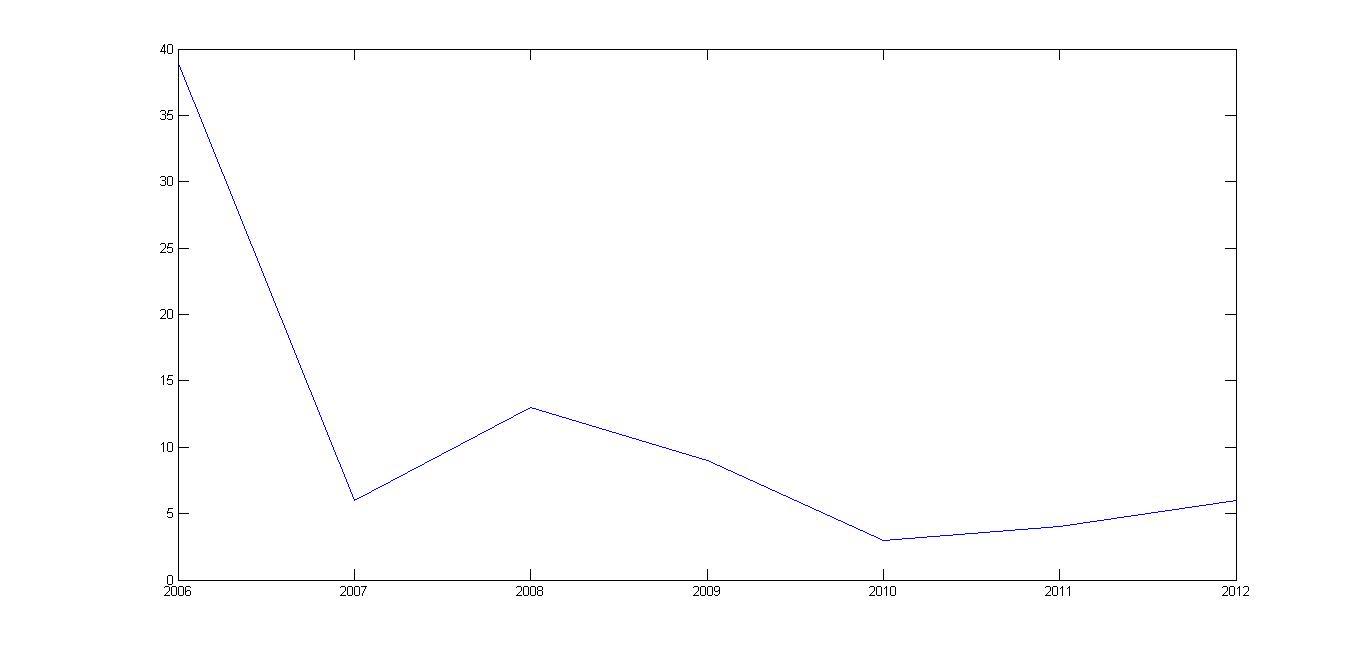
\includegraphics[width=\textwidth]{indultosporanho.jpg}


% \end{enumerate}

\item (40 pt) Considere la funci\'on
$$
f(x)=
\begin{cases}
\frac{cos(x)}{x} \quad  \text{, si } x\in\,[-5,0[\\
\frac{sin(x)}{x} \quad  \text{, si } x\in\,]0,5[
\end{cases}.
$$
En una misma figura grafique las funciones dadas por $f(x)$, $f(f(x))$, $f(x+1)$ y $f(x^2+1)$. Grabe esta im\'agen como \texttt{funciones.jpg} y adj\'untela al correo.

\textbf{Desarrollo:}

% Debido a al composici\'on nos conviene usar un fichero tipo \texttt{function} para trabajar este problema, creamos
% \begin{lstlisting}
% function y=f(x)
% for i=1:length(x)
% 	if(x(i)>=-5 && x(i)<0)
%     	y(i)=cos(x(i))/x(i);
%     elseif (x(i)>=0 && x(i)<5)
%        y(i)=sin(x(i))/x(i);
%     end
% end
% end
% \end{lstlisting}
% y graficamos con el rutero
% \begin{lstlisting}
% x=linspace(-5,4.9,123);
% figure(1);
% subplot(2,2,1);
% plot(x,f(x));
% subplot(2,2,2);
% plot(x,f(f(x)));
% subplot(2,2,3);
% x=-6:0.1:3.99;
% plot(x,f(x+1));
% subplot(2,2,4);
% x=-sqrt(4):0.1:sqrt(3.9);
% plot(x,f(x.^2+1));
% \end{lstlisting}
% lo que genera la gr\'afica solicitada

% 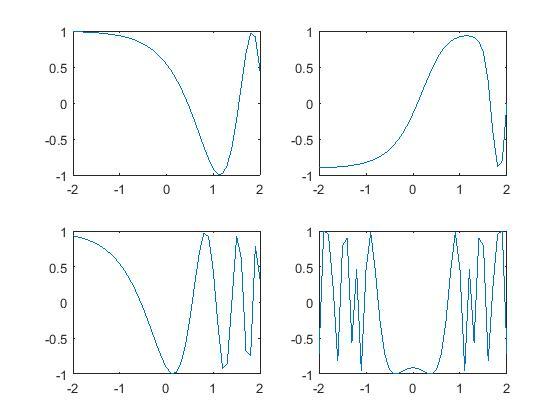
\includegraphics[width=\textwidth]{funciones.jpg}

\end{enumerate}
\end{document}   